\section{Method}
\label{sec:method}

We aim to enhance 3D LiDAR scene generation by combining rich 3D representations with pretrained RGB image priors learned from large-scale image datasets. 

\NS{
To exploit the knowledge learned from large-scale RGB image dataset, we initialize our latent FM model with weights pretrained on such data.
} 
\begin{figure}[t!]
\centering
\def\svgwidth{0.99\linewidth} 
\input{pipeline_l.pdf_tex}
\caption{\textbf{End-to-end training.} We jointly train the VAE and the flow matching (FM) model with the additional alignment loss $\mathcal{L}_{\textrm{Alignment}}$, which aligns the internal representations of the FM model with 3D point features $y$. At each step, the VAE is updated with $\mathcal{L}_{\textrm{AE}} + \lambda_1 \mathcal{L}_{\textrm{Alignment}}$, followed by updating the FM model with $\mathcal{L}_{\textrm{Denoising}} + \lambda_2 \mathcal{L}_{\textrm{Alignment}}$.
$z_t$ is the interpolated noisy latent vector derived from the clean latent $z$.
The input point cloud and its associated features are projected onto the range image $x$ and the feature map $y$, respectively, using an equirectangular projection.
}
\label{fig:pipeline}
\end{figure}
However, directly fine-tuning from \NS{pretrained} weights causes a collapse of prior knowledge due to the domain gap between natural-image latents and range-image latents.
To address this issue, we introduce a VAE alignment training recipe, which is guided by 3D representation alignment for cross-modality adaptation.
We call this unified framework \ours, which operates on range images while leveraging both 2D priors from natural images and 3D representation alignment. 
An overview of our framework is shown in Figure~\ref{fig:tuning}.

In \ours, 3D representations from a 3D pretrained backbone are used to compute an alignment loss that supervises the internal activations of the FM model. The first stage, VAE alignment, freezes the initialized FM model while training the VAE from scratch. Guided by the alignment loss, the VAE adapts its latent space to the input space of the FM model. In the second stage, end-to-end training, we apply joint alignment: the alignment loss propagates gradients to both the VAE and the FM model, ensuring that the autoencoder also benefits from a FM model signal rather than leaving the adaptation solely to the FM model. We illustrate our end-to-end training in Figure~\ref{fig:pipeline}.

For the alignment loss, each LiDAR point cloud is encoded with a pretrained 3D feature extractor to obtain point-level self-supervised features. An equirectangular projection then maps the unstructured point cloud into a 2D feature grid that is geometrically aligned with the FM model’s internal representations. This process distills knowledge from the pretrained 3D foundation model and establishes a shared, expressive latent space between the VAE and the FM model.

\subsection{Preliminaries}
This section provides the necessary background for our method. Following prior work \cite{rombach_high-resolution_2022,hu_rangeldm_2024,ran_towards_2024}, we generate LiDAR point clouds by applying FM in the latent space of a VAE.

\textbf{Equirectangular Projection.}
We represent unstructured point clouds as range images where pixel coordinates come from discretized yaw and pitch, pixel values store depth, and only the closest point is kept per pixel.
This representation, while not being lossless, allows a much faster processing. 
More precisely, the pixel coordinate  $(i,j)$ of a point $(p_x,p_y,p_z)$  projected onto a grid of size $H$x$W$ are
\begin{equation}
\begin{pmatrix}
i \\
j
\end{pmatrix}
=
\begin{pmatrix}
\left( 1 - \left( \arcsin(p_z/ r) + f_{\text{down}} \right) f_v^{-1} \right) H
\\
\frac{1}{2}\left(1 - \arctan(p_y/p_x) \pi^{-1}\right) W
\end{pmatrix}
\label{eq:proj}
\end{equation}
where $f_v = |f_{up} - f_{down}|$ is the vertical field of view of the LiDAR sensor and $r=\sqrt{p_x^2+p_y^2+p_z^2}$ is the depth.

\textbf{VAE Training.}
We adopt the VAE architecture of~\cite{ran_towards_2024}, which uses horizontal kernels \NS{and circular padding} in convolution and downsampling layers to account for the wide aspect ratio of LiDAR range images.  
\NS{We encode range image $x$ with encoder $\mathcal{E}$ to a compact latent vector $z=\mathcal{E}
(x)$} with downsampled spatial dimensions and an upsampled channel dimension. Overall, the smaller dimension of the latent space makes the denoising process faster. 
We decode with $\mathcal{D}$ latent vector z to produce $\hat{x} = \mathcal{D}(z)=\mathcal{D}(\mathcal{E}(x))$ a reconstructed range image.

The overall VAE objective is $\mathcal{L}_{\text{AE}} = \mathcal{L}_{\text{MSE}} + \mathcal{L}_{\text{KL}} + \mathcal{L}_{\text{GAN}}$ similar to~\cite{rombach_high-resolution_2022}.  The reconstruction loss $\mathcal{L}_{\text{MSE}}$ is computed between the input range image $x$ and its reconstruction $\hat{x}$. The term $\mathcal{L}_{\text{KL}}$ enforces the encoder's latent distribution to remain close to a Gaussian prior, ensuring a smooth and sampling-friendly latent space. To mitigate the typical blurriness of VAE outputs, we also include an adversarial loss $\mathcal{L}_{\text{GAN}}$, which uses a patch-wise discriminator to encourage realistic and sharp reconstructions, as motivated by \cite{nakashima_fast_2025}. The discriminator is implemented as a convolutional network and trained jointly with the VAE.  


\textbf{LiDAR Scene Generation with Flow Matching.}
We generate LiDAR scenes by producing latent representations with a stochastic interpolant~\cite{ma_sit_2024}, which are subsequently decoded into range images. These range images are then unprojected to obtain point clouds.


Stochastic interpolants unify flow- and diffusion-based generative models~\cite{albergo2023stochastic}. In our work, we adopt a simple linear interpolation process that gradually transforms noise $\varepsilon\sim\mathcal{N}(\mathbf{0},\mathbf{I})$ into latent data $\mathbf{z}_*\sim p(z)$ in reverse time, defined as $z_t = (1-t)\mathbf{z}_*+t\varepsilon$ with $ t\in[0,1]$. The target $\mathbf{z}_*$ can then be generated either deterministically or stochastically, using an ordinary or a stochastic differential equation, respectively. In both cases, only a single estimator of the velocity field is required, given by $ \mathbf{v}(z,t) = \mathbb{E}[\varepsilon-\mathbf{z}_*|z_t=z]$. We optimize our FM network $v$ to be an estimator of $\mathbf{v}$ with the following objective $\mathcal{L}_{\text{Denoising}} = \mathbb{E}[\|v(z_t,t)-(\varepsilon - \mathbf{z}_*)\|^2]$
We parametrize the estimator of the vector field using a transformer architecture. 
 
\subsection{R3DPA}

\textbf{3D Representation Alignment.}
The goal of representation alignment is to supervise the internal representations of FM transformers using features extracted from a pretrained encoder. 
Following~\cite{wang_repa_2025, leng_repa-e_2025}, we first project the transformer output from the middle layer into a feature map of size $H \times W$ using a projection layer. 
We then extract 3D point features from the corresponding LiDAR scene using a pretrained 3D backbone. However, these 3D point features are not directly usable due to their large number and unstructured nature.  
We therefore project them onto a grid using an equirectangular projection (\ref{eq:proj}), with the grid size matching the spatial dimensions of projection layer output.
Points falling into the same grid cell are averaged, resulting in a feature grid $y \in \mathbb{R}^{H \times W \times D}$ where $D$ is the dimension of 3D features. 
Figure \ref{fig:scalr_features} shows a PCA visualization of projected features. 
Since each grid cell can be mapped one-to-one to a FM token, the alignment loss can be applied as follows: 

\begin{equation}
\mathcal{L}_{\textrm{Alignment}}(\theta,\phi) = -\mathbb{E} \Bigg[ \frac{1}{H} \frac{1}{W} \sum_{j=1}^H \sum_{i=1}^W \langle y_{(i,j)}, y_{(i,j)}^t \rangle \Bigg], 
\label{eq:align}
\end{equation}

Here, $y \in \mathbb{R}^{H \times W \times D}$ denotes the normalized and projected 3D features, 
while $y^t$ is the normalized  and projected internal representation of the model from noisy latent at timestep $t$,  
$\theta$ is the parameters of the FM model and $\phi$ is the parameters of the projection head.

\begin{figure}[t!]
    \centering
    \begin{minipage}{0.9\columnwidth}
        \centering
        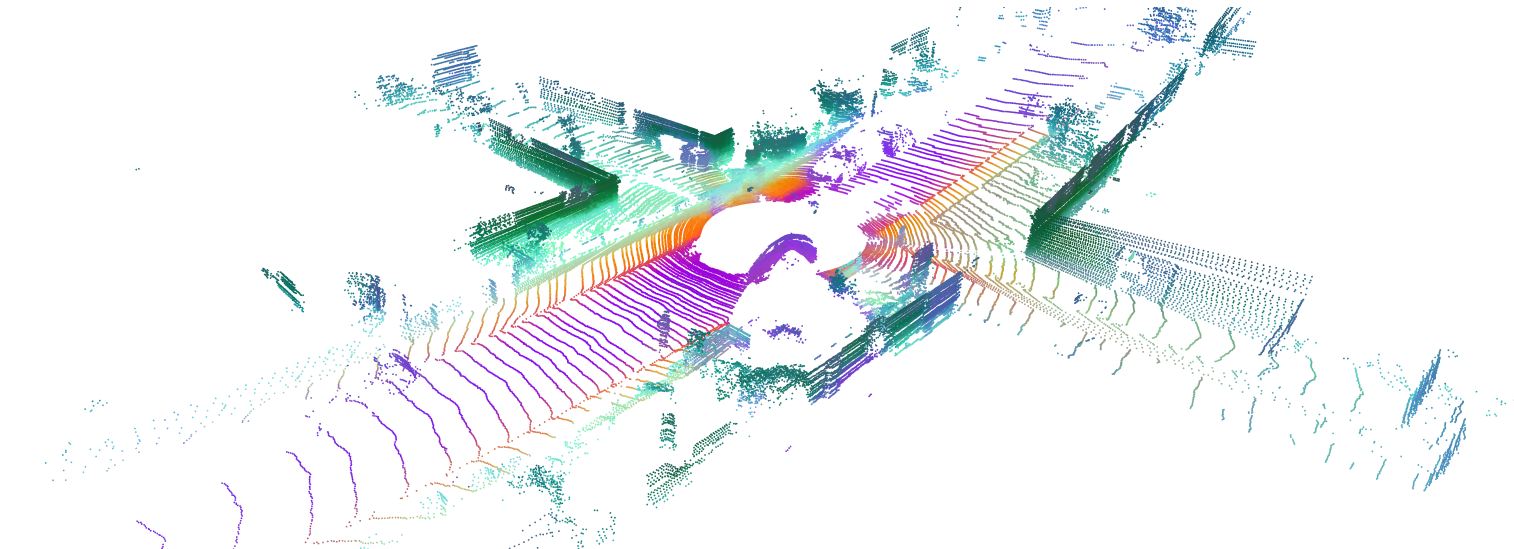
\includegraphics[width=\linewidth]{figures/scalr_pc.png}
        \label{fig:mask}
    \end{minipage}
    \hfill
    \begin{minipage}{0.9\columnwidth}
        \centering
        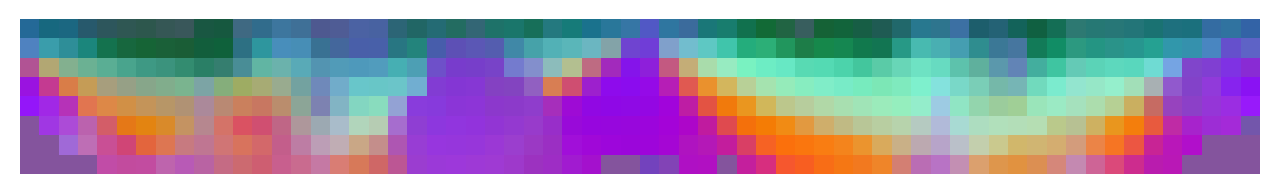
\includegraphics[width=\linewidth]{figures/scalr8x64.png}
    \end{minipage}
    \caption{\textbf{PCA visualization of 3D features and their projection.} The 768-dimensional 3D features \cite{puy2024three} are reduced to three principal components, which are then mapped to RGB colors for visualization.
    (Top) Point features in LiDAR scene, (Bottom) Projected features at grid size 8$\times$64, matching the internal representation of the transformer \cite{ma_sit_2024}.}
    \label{fig:scalr_features}
\end{figure}


 \begin{figure*}[t!]
    \centering
    \begin{tabular}{ccc}
        % Column 1
        \begin{minipage}{0.49\textwidth}
            \vspace{+0.25em}
            \centering
            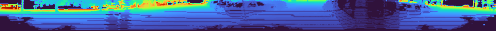
\includegraphics[width=\linewidth]{figures/latents/range_image_0.png} \\[0.5ex]
            
\includegraphics[width=\linewidth]{figures/latents/range_image_500.png} \\[0.5ex]
            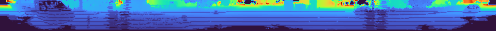
\includegraphics[width=\linewidth]{figures/latents/range_image_600.png} \\[0.5ex]
            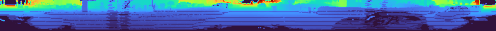
\includegraphics[width=\linewidth]{figures/latents/range_image_900.png} \\[0.5ex]
            \small \textrm{Range Images}
        \end{minipage}
        \begin{minipage}{0.24\textwidth}
            \centering
            
\includegraphics[width=\linewidth]{figures/latents/pca_latent_scratch_0.png} \\[0.5ex]
            
\includegraphics[width=\linewidth]{figures/latents/pca_latent_scratch_500.png} \\[0.5ex]
            
\includegraphics[width=\linewidth]{figures/latents/pca_latent_scratch_600.png} \\[0.5ex]
            
\includegraphics[width=\linewidth]{figures/latents/pca_latent_scratch_900.png} \\[0.5ex]
            \small \textrm{Standard VAE latents}
        \end{minipage}
        \begin{minipage}{0.24\textwidth}
            \centering
            
\includegraphics[width=\linewidth]{figures/latents/pca_latent_e2e_0.png} \\[0.5ex]
            
\includegraphics[width=\linewidth]{figures/latents/pca_latent_e2e_500.png} \\[0.5ex]
            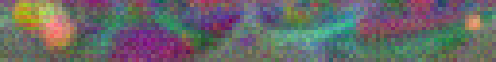
\includegraphics[width=\linewidth]{figures/latents/pca_latent_e2e_600.png} \\[0.5ex]
            
\includegraphics[width=\linewidth]{figures/latents/pca_latent_e2e_900.png} \\[0.5ex]
            \small \textrm{End-to-end VAE latents}
        \end{minipage} \\
    \end{tabular}
    \caption{\textbf{Effect of end-to-end training on latents.} (Left) Input range images. (Middle) Corresponding PCA visualizations of latents obtained using the standard VAE paradigm, such as \cite{ran_towards_2024}, where the VAE is trained independently on range images. (Right) PCA visualizations of latents from our end-to-end training with 3D representation alignment. Latents obtained through end-to-end training are more expressive, allowing a clear distinction of objects and background in the scene.}
    \label{fig:latent_visu}
\vspace{-0.5cm}
\end{figure*}


%%%%%%%%%%%%%%%%%%%%%%%%%%% 
\textbf{VAE Alignment for RGB Image Priors.}
Our VAE alignment step enables us to exploit natural image pretrained FM model weights by transferring their knowledge to range images, which are limited in dataset size.  
To this end, we initialize our model with the weights of a FM model trained on the same backbone using a significantly larger dataset of natural images. 
However, we observe that directly training with these weights yields no performance gain (see Table \ref{tab:abl_vae}), which is expected given the domain gap between natural-image latents and range-image latents. 
To address this, we introduce VAE alignment: the FM model is initialized with RGB image pretrained weights, with the exception of the feature projection head and the first layer of the transformer patch embedding, which is trained to resolve the latent channel mismatch, while the rest of the model is kept frozen and only the VAE is trained. 
\SG{During training, we include the alignment loss (\ref{eq:align}) to the VAE training and use it as a guidance signal from the generative model to the encoder. This signal enforces the VAE to align with the internal representations of the pretrained FM backbone.} Once this step is complete, we unfreeze the FM model and proceed with full end-to-end training.
 

\textbf{End-to-end training.} End-to-end training jointly optimizes the VAE and the FM model (see Figure~\ref{fig:pipeline}).
During joint optimization, the VAE and SiT networks are updated with their respective objectives, both combined with $\mathcal{L}_{\text{Alignment}}$. Concretely, we optimize at each step (i) the VAE with $\mathcal{L}_{\text{AE}} + \lambda_1 \mathcal{L}_{\text{Alignment}}$, where $\mathcal{L}_{\text{Alignment}}$ updates only the encoder weights of VAE, and (ii) the FM model with $\mathcal{L}_{\text{Denoising}} + \lambda_2 \mathcal{L}_{\text{Alignment}}$.

FM models are typically trained in a space normalized to unit variance. Since the VAE latent space evolves during training, we follow~\cite{leng_repa-e_2025} and normalize the transformer input with a batch normalization layer. At inference, we fix the normalization using statistics accumulated with an exponential moving average.

End-to-end training improves alignment between the encoder and the FM model, leading to a more expressive latent space (see Figure~\ref{fig:latent_visu}) and higher generation quality.
